\chapter{Определение позы человека в видеопоследовательности} \label{chapt6}

В этой главе я рассматриваю задачу определения позы человека в видеопоследовательности. Как описано в обзоре \ref{chapt-related::human_pose_definithion}, в настоящий момент научное сообщество определяет позу человека на изображении как положение его $K$ суставов. Таким образом, позой человека в момент времени $t$ является последовательность точек $P^t \in \left\{ \left\{p_i^t\right\}_{i=1}^K | p_i^t \in \mathbb{R}^2\right\}$ на изображении.

В своей работе я рассматриваю алгоритм определения позы человека в качестве следующего этапа обработки видеоданных после сопровождения. Поэтому моя постановка задачи определения позы в видеопоследовательности имеет следующий вид:
\begin{itemize}
	\item[Вход:] видеопоследовательность $I=\left\{I_t\right\}_{i=1}^N$;
	\item[Выход:] поза человека на каждом кадре $P=\left\{P^t\right\}_{t=1}^{N}$.
\end{itemize}

\section{Математическая модель наблюдаемых данных}

Я рассматриваю определение позы человека в видео как задачу минимизации функции энергии $E(P, \Theta|I)$, где $\Theta$ "--- скрытые параметры модели. Параметр $\Theta$ может включать как скрытые параметры позы человека на одно кадре (например, параметр размера), так и глобальные параметры модели человека (цветовая модель). Можно считать, что функция энергии $E(P, \Theta|I)$ задаёт ненормированную функцию правдоподобия позы в видеопоследовательности в виде $\tilde{p}(P, \Theta|I) = \exp\left(-E(P, \Theta|I)\right)$. В дальнейшем для упрощения выкладок я буду неявно предполагать зависимость функции энергии от исходной видеопоследовательности, т.~е. $E(P, \Theta) = E(P, \Theta|I)$.

Используемая модель наблюдаемых данных является обобщением модели позы человека на изображении на случай видеопоследовательности. Для этого базовая модель расширяется предположением о зависимости позы человека на разных кадрах. Стандартный подход к расширению модели позы человека на случай видеопоследовательности соответствует следующей функции энергии:
\begin{equation}
	\begin{aligned}
		E(P, \Theta) &= \sum_{t=1}^T E_I(P^t, \Theta) + \sum_{t=1}^{T-1}E_T(P^{t+1}, P^{t}, \Theta),
	\end{aligned}
\end{equation}
где $E_I(P^t)$ "--- модель позы человека на кадре \eqref{eq::frame}, а $E_T(P^{t+1}, P^{t})$ "--- модель изменения позы между кадрами. Такую модель можно рассматривать как марковскую цепь первого порядка, где состояние в каждый момент времени является многомерной величиной и описывает позу человека.

Она состоит из двух частей: 1) базовая модели позы человека на изображении $E_I(P^t, \Theta)$ и 2) модель движения её суставов $E_T(P^{t+1}, P^{t}, \Theta)$.

\subsection{Модель позы человека на изображении}

Согласно обзору существующих методов в научных работах представлены две основные модели позы человека: модель из набора деформируемых частей и регрессионная модель позы.

Несмотря на то, что регрессионная модель на момент написания данной диссертации позволяет добиться лучших результатов определения позы на изображении, её обобщение на случай видеопоследовательности затруднено. Построенное отображение входного изображения $I_t$ на позу человека $P^t$ на нем не позволяет использовать априорные сведения, полученные на соседних кадрах.

Поэтому в качестве базовой модели позы человека на изображении была выбрана модель из набора деформируемых частей. Соответствующая ей марковская сеть, определяет ненормированную функцию правдоподобия $\tilde{p}(P^t, \Theta^t) = \exp(-E_I(P^t, \Theta))$. Это свойство позволяет интегрировать её как часть большей графической модели, используя информацию с предыдущих кадров для построения априорных ограничений.

Модель из набора частей описывается с помощью функции энергии $E_I(P^t, \Theta^t)$, минимум которой определяется в качестве позы человека на изображении $I_t$:
\begin{equation}
	E_I(P^t, \Theta) = \sum_{i=1}^K{\phi_i(p_i^t, s^t)} + \sum_{\left(i,j\right)\in E}{\psi_{(i,j)}^s(p_i^t, p_j^t, s^t)},
	\label{eq::frame}
\end{equation}

Унарный потенциал $\phi_i(p_i^t, s^t)$ можно рассматривать, как отклик алгоритма обнаружения сустава человека на заданном масштабе изображения. Парный потенциал $\psi_{(i,j)}^s(p_i^t, p_j^t, s^t)$ задаётся в виде квадратичной формы, зависящей от смещения между суставами. Функция энергии зависит от параметра размера человека $s^t$ на текущем изображении, и не зависит от остальных скрытых параметров модели.

На практике параметр положения $p^t$ суставов является дискретной величиной, определённой на изображении с некоторым шагом. Параметр размера $s^t$ также является дискретным и соответствует разным масштабам при обнаружении суставов.

\subsection{Модель движения}

Наиболее простым способом задания модели изменения позы является предположение о независимости движения суставов:
\begin{equation}
	E_T(P^{t+1}, P^{t}, \Theta) = \sum_{i=1}^K\psi_i^t(p_i^{t+1}, p_i^t, \Theta)
\end{equation}

Так как модели движения разных суставов схожи, то достаточно рассмотреть её лишь для одного из них. Для упрощения обозначений в данном подразделе я опускаю индекс рассматриваемого сустава. Например, $p^t$ используется для обозначения состояния рассматриваемого сустава на кадре $I_t$.

Такое расширение модели позы человека на изображении на случай видеопоследовательности использовался также в предыдущих работах. Например, в работе \cite{park2011n} предлагалась модель движения, предполагающее слабое изменение позы человека между кадрами:
\begin{equation*}
	\psi^t(p^{t+1}, p^t, \Theta) = \frac{1} {2 {s^t}^2}(p^{t+1} - p^t)^{T-1} \left(\Sigma_p^p\right)^{-1} (p^{t+1} - p^t)
\end{equation*}
Таким образом, оптимальное значение такой модели движения достигается при постоянстве позы человека в видео. Изменение позы при движении оказывается <<допустимым шумом>>.

В этой работе я расширил эту модель движения. Я использовал линейную динамическую систему для описания движения суставов тела человека. Для этого скрытое состояние $\Theta$ модели было расширено характеристикой движения каждого сустава. В работе я рассматриваю линейную модель движения суставов, т.~e. состояние каждого сустава описывается его положением $p^t$ на кадре и мгновенной скоростью движения $v^t \in \mathbb{R}^2$. По аналогии с позой человека, я обозначаю скорость всех суставов в видеопоследовательности через $V$. Если обозначить через $h^t = [p^t, v^t]$ "--- состояние рассматриваемого сустава позы человека на кадре $t$, то предложенная модель движения принимает вид:
\begin{equation}
	\begin{aligned}
		\psi^t(p^{t+1}, p^{t}, \Theta) &=
			\frac{1}{2 {s^t}^2} (h^{t+1} - A h^t)^T \Sigma_p^{-1} (h^{t+1} - A h^t) \\
		A &=
			\begin{bmatrix}
			1 & 0 & 1 & 0 \\
			0 & 1 & 0 & 1 \\
			0 & 0 & 1 & 0 \\
			0 & 0 & 0 & 1 \\
			\end{bmatrix} \\
	\label{eq::temp}
	\end{aligned}
\end{equation}

Допустимое отклонение от линейной модели движения задается симметричной положительно определенной матрицей $\Sigma_p \in \mathbb{S_+}$. Для уменьшения количества параметров я рассматривал только диагональные матрицы $\Sigma_p$ следующего вида:
\begin{equation}
	\begin{aligned}
		\Sigma_p &= \left[
			\begin{array}{c|c}
			\Sigma_p^p & \Theta \\ \hline
			\Theta     & \Sigma_p^v
			\end{array}
			\right] \\
		\Sigma_p^p &= \alpha_p^{-1} I_{2\times2} \\
		\Sigma_p^v &= \alpha_v^{-1} I_{2\times2} \\
		\alpha_p &> 0, \alpha_v > 0,
		\label{eq::sigma}
	\end{aligned}
\end{equation}
Матрица $\Sigma_p^p$ описывает допустимое отклонение положения сустава $p^{t+1}$ от его линейного предсказания $p^t + v^t$, a $\Sigma_p^v$ "--- допустимое изменение скорости сустава между кадрами.

Без дополнительной регуляризации модель движения \eqref{eq::temp} допускает неправдоподобно большое значение скорости движения сустава, так как ограничивает только её изменение. Для решения этой проблемы был добавлен фактор, задающий априорное предпочтение на скорость движения суставов на первом кадре:
\begin{equation}
	\begin{aligned}
		\psi^0(v^1) &= \frac{1}{2 {s^1}^2}{v^1}^T \left({\Sigma_p^{v^1}}\right)^{-1} v^1 \\
		\Sigma_p^{v^1} &= \alpha_{v^1}^{-1} I_{2\times2}
	\end{aligned}
\end{equation}

Также моя модель ограничивает неправдоподобное изменение размера человека между кадрами:
\begin{equation}
	\eta^t(s^{t+1}, s^t) = \frac{1}{2} \left(\frac{s^{t+1} - s^t}{s^t\sigma_s}\right)^2
\end{equation}

Таким образом, предложенная модель движения имеет следующий вид:
\begin{equation}
	\sum_{t=1}^{T-1}{\Psi(P^{t+1}, P^t)} = 
		\sum_{i=1}^K\left(\psi^0_i(v^1_i) + \sum_{t=1}^{T-1}\psi_i^t(h_i^{t+1}, h_i^{t}, \Theta) \right) + \sum_{t=1}^{T-1} \eta^t(s^{t+1}, s^{t})
	\label{eq::motion_model}
\end{equation}

\subsection{Частные случаи}

Предложенная модель имеет два интересных частных случая, рассматриваемых в предыдущих работах.

Рассмотрим случай, когда $\alpha_v \rightarrow +\infty, \alpha_{v^1} \rightarrow +\infty$ и $\sigma_s \rightarrow +\infty$. Этот случай описывает значительное увеличение энергии в случаях, когда значение скорости какого-либо сустава отлично от $0$:
\begin{equation}
	\begin{aligned}
		\lim_{\alpha_{v^1} \rightarrow +\infty}{\argmin_{v^1} \psi^0(v^1)} &= 0 \\
		\lim_{\alpha_{v} \rightarrow +\infty}{\argmin_{v^t} \psi^t(h_i^{t+1}, h_i^{t}, \Theta)} &= 0 \\
		\lim_{\sigma_s \rightarrow +\infty}{\eta^t(s^{t+1},s^t)} &= 0
	\end{aligned}
\end{equation}
То есть оптимальным является решение, где все параметры скорости равны 0. При этом условии модель движения суставов имеет вид:
\begin{equation}
	\begin{aligned}
		\psi^t(h_i^{t+1}, h_i^{t}, \Theta) |_{v^t = v^{t+1} = 0} &= \frac{1} {2 {s^t}^2}(p^{t+1} - p^t)^T \left(\Sigma_p^p\right)^{-1} (p^{t+1} - p^t) \\
		\psi^0(v^1)|_{v^1=0} &= 0
	\end{aligned}
\end{equation}
То есть предложенная модель становится эквивалентной модели движения, описанной в работе \cite{park2011n}.

Рассмотрим другой частный случай. Если ослабить ограничения на небольшое изменение скорости суставов между кадрами, то модель \eqref{eq::motion_model} описывает независимое определение позы человека на каждом кадре. Действительно
\begin{equation}
	\begin{aligned}
		\lim_{\alpha_{v} \rightarrow 0+0}{\psi^t(h_i^{t+1}, h_i^{t}, \Theta)} &= 0 \\
		\lim_{\alpha_{v^1} \rightarrow 0+0}{\psi^0(v^1)} &= 0 \\
		\lim_{\sigma_s \rightarrow +\infty}{\eta^t(s^{t+1},s^t)} &= 0
	\end{aligned}
\end{equation}
То есть графическая модель распадается на независимые связные компоненты, соответствующие позе человека на каждом кадре.

\section{Метод оптимизации}

\subsection{Анализ модели}

\label{subsec::model_analysis}

Для описания предложенного алгоритма оптимизации важно рассмотреть две задачи, связанные с функцией представленной функции энергии:
\begin{enumerate}
	\item определение скорости суставов при известных позе и росте человека человека в видео "--- $\argmin_{V} E(P, \Theta)$;
	\item определение позы и размера человека на кадре $t$ при известных остальных параметрах модели "--- $\argmin_{P^t, s^t} E(P, \Theta)$.
\end{enumerate}

\subsubsection{Определение скорости}

Рассмотрим задачу определение скорости движения суставов при известных позе и росте человека в видео $V = \argmin_{V} E(P, \Theta)$. Модель позы человека на изображении $E_I(P^t, \Theta)$ и модель изменения размера $\eta^t(s^{t+1}, s^t)$ не зависят от параметров скорости. Поэтому рассматриваемая задача эквивалентна задаче оптимизации:
\begin{equation}
	V = \argmin_V E(V|P, \Theta_{\backslash V}) = \argmin_V {\sum_{i=1}^K\left(\psi^0_i(v^1_i) + \sum_{t=1}^{T-1}\psi_i^t(h_i^{t+1}, h_i^{t}, \Theta) \right)}
\end{equation}
Из этой формы видно, что скорости разных суставов никогда не входят в одно слагаемое, а значит можно проводить оптимизацию скорости каждого сустава независимо:
\begin{equation}
	\begin{aligned}
		V_i &= \argmin_{V_i} \psi^0_i(v^1_i) + \sum_{t=1}^{T-1}\psi_i^t(h_i^{t+1}, h_i^{t}, \Theta) \\
		V &= \cup_{i=1}^K V_i
	\end{aligned}
\end{equation}

Рассмотрим поиск оптимального значения для скорости одного сустава. В дальнейшем для упрощения выкладок я буду опускать индекс текущего сустава. Учитывая \eqref{eq::temp} и \eqref{eq::sigma}, оптимизируемую энергию $E(V|P, \Theta_{\backslash V})$ можно переписать в виде суммы унарных и парных потенциалов:
\begin{equation}
	\begin{aligned}
		E(V|P, \Theta_{\backslash V}) &= \psi^0(v^1) + \sum_{t=1}^{T-1} \left( \psi^{t,u}(v^t|p^{t+1}, p^{t}, s^t) + \psi^{t,p}(v^{t+1}, v^{t}|s^t) \right) \\		
		\psi^{t,u}(v^t|p^{t+1}, p^{t}, s^t) &= \frac{(\Delta p^t - A^u v^t)^T {\Sigma_p^p}^{-1} (\Delta p^t - A^u v^t)} {2 {s^t}^2} \\
		\psi^{t,p}(v^{t+1}, v^{t}|s^t) &= -\frac{(v^{t+1} - A^p v^t)^T {\Sigma_p^v}^{-1} (v^{t+1} - A^p v^t)} {2 {s^t}^2} \\ 
		\Delta p^t &= p^{t+1} - A_p^u p^t \\
		A &= \left[
		\begin{array}{c|c}
		A_p^u  & A^u \\ \hline
		\Theta & A^p
		\end{array}
		\right] \quad
		A_p^u, A^u, A^p \in \mathbb{R}^{2 \times 2}
	\end{aligned}
\end{equation}

В данной постановке задача поиска минимума функции энергии $E(V|P, \Theta_{\backslash V})$ совпадает с задачей определения состояний линейной динамической системы (ЛДС):
\begin{equation}
\begin{aligned}
	V &= \argmax_V {p\left(V | \left\{\Delta p^t\right\}_{t=1}^{T-1}, \left\{s^t\right\}_{t=1}^T\right)} \\ 
	\Delta p^t &\sim N(A^u v^t, (s^t)^2\Sigma_p^p) \\
	v^{t+1} &\sim N(A^p v^t, (s^t)^2\Sigma_p^v) \\
	v^1 &\sim N(\Theta, (s^t)^2\Sigma_p^{v^1}) \\
	v^T &= A^p v^{T-1}
\end{aligned}
\end{equation}
Поиск наиболее вероятной конфигурации $V$ осуществляется с помощью фильтра Калмана и РТС уравнений.

\subsubsection{Определение позы и размера на кадре}

Рассмотрим задачу определения позы $P^t$ и размера $s^t$ человека на некотором кадре при известных остальных параметрах модели $\argmin_{P^t, s^t} E(P, \Theta)$:
\begin{multline}
	E(P^t, s^t| P^{\backslash t}, \Theta_{\backslash s^t}) = E(P, \Theta)\bigg\rvert_{P^{\backslash t}, \Theta_{\backslash s^t}} = \\ = \left(\sum_{t'=1}^T{E_I(P^{t'}, \Theta)} + \sum_{t'=1}^{T-1}{E_T(P^{t'+1}, P^{t'}, \Theta)}\right)\bigg\rvert_{P^{\backslash t}, \Theta_{\backslash s^t}}
\end{multline}

Модель позы человека в видео является марковской цепью первого порядка, поэтому рассматриваемая энергия имеет вид:
\begin{multline}
	E(P^t, s^t| P^{\backslash t}, \Theta_{\backslash s^t}) = E_I(P^{t}, \Theta) + \\ + \left(E_T(P^{t+1}, P^{t}, \Theta) + E_T(P^{t}, P^{t-1}, \Theta)\right)\bigg\rvert_{\substack{P^{t-1}, P^{t+1}, \\ s^{t-1}, s^{t+1}, \\ V^{t-1}, V^{t+1}}} + C,
\end{multline}
где $C$ "--- константа, не зависящая от рассматриваемых параметров. Чтобы не рассматривать отдельно случаи граничные случаи, можно определить состояние модели в моменты времени $t=0$ и $t=T+1$ значениями в моменты времени $t=1$ и $t=T$ соответственно.

Учитывая \eqref{eq::frame} и \eqref{eq::temp}, рассматриваемая энергия имеет вид:
\begin{multline}
	E(P^t, s^t| P^{\backslash t}, \Theta_{\backslash s^t}) =
	 \sum_{i=1}^K{
	 	\left(\underbrace{\phi_i(p_i^t, s^t) +
	 		 \psi_i^t(h_i^{t+1}, h_i^{t}, \Theta) +
	 		 \psi_i^t(h_i^{t}, h_i^{t-1}, \Theta)}_{\phi'_i(p_i^t, s^t)} \right)} + \\ +
 		  \sum_{\left(i,j\right)\in E}{
 		  	\psi_{(i,j)}^s(p_i^t, p_j^t, s^t)} +
 	  	  \underbrace{\eta^t(s^{t+1}, s^{t}) + \eta^t(s^{t}, s^{t-1}) + C'}_{\phi_s(s^t)}
\end{multline}

Таким образом, условная модель человека $E(P^t, s^t| P^{\backslash t}, \Theta_{\backslash s^t})$ на кадре $I_t$ для каждого масштаба $s^t$ представляет сумму унарных $\phi'_i(p_i^t, s^t)$ и парных $\psi^s_{(i,j)}(p_i^t, p_j^t, s^t)$ потенциалов относительно положения суставов позы человека. Так как модель движения не добавляет парных потенциалов в энергию $E(P^t, s^t| P^{\backslash t}, \Theta_{\backslash s^t})$, то эта энергия факторизуется согласно той же графической модели, что и модель позы $E_I(P^t, \Theta)$. Факторы $\eta^t(s^{t+1}, s^t)$ и $\eta^t(s^t, s^{t-1})$ задают апостериорное предпочтение на значение параметра размера позы.

Таким образом, условная модель позы человека $E(P^t, s^t| P^{\backslash t}, \Theta_{\backslash s^t})$ является обобщением модели позы человека на изображении $E_I(P^t, \Theta)$. Так как при оптимизации модели $E_I(P^t, \Theta)$ алгоритмы производят перебор по различным значениям параметра размера человека $s^t$, то для условной модели позы человека также выполняются свойства:
\begin{enumerate}
	\item вычислительная сложность алгоритма поиска глобального оптимума равна $\mathcal{O}(KM)$;
	\item алгоритм построения множества наилучших гипотез позы человека на изображении, отличающихся не менее чем на заданную величину равна имеет сложность $\mathcal{O}(KM)$.
\end{enumerate}

\subsubsection{Сложность поиска глобального оптимума}

Каждой функции энергии, описывающей модель позы человека, соответствует марковская сеть. От её свойств зависит сложность алгоритмов поиска оптимального значения модели. В общем случае поиск глобального оптимума в графических моделях осуществляется алгоритмом распространения доверия. Его вычислительная сложность зависит от количества допустимых состояний минимальной группы вершин, разделяющих графическую модель на две части. Если графическая модель является деревом, то сложность алгоритма квадратично зависит от количества допустимых состояний для каждой вершины. Примером такой графической модели является модель позы человека на изображении при условии известного параметра масштаба. Специальный вид парных потенциалов, позволил сократить сложность вывода в графической модели до линейной зависимости от количества допустимых положений суставов на изображении.

К сожалению, при расширении этой модели, в марковской сети появляются циклы, а следовательно сложность поиска оптимального решения существенно возрастает. На рисунке \ref{} представлена графическая модель, соответствующая модели \cite{park2011n}. Её можно рассматривать как марковскую цепь первого порядка, где каждое состояние описывается множеством вершин одного кадра.

Рассмотрим вычислительную сложность алгоритма поиска глобального минимума для такой марковской цепи. Если на кадре имеется $M$ возможных положений каждого сустав, то сложность алгоритма распространения доверия равна $\mathcal{O}(M^{K}T)$. Здесь существенно использован факт, что модель движения \eqref{eq::motion_model} является квадратичной формой, и для вычисления сообщений в сети может быть использован метод дистантного преобразования. Таким образом, сложность поиска оптимального множества поз линейно зависит от количества возможных поз человека на изображении. Так как значение параметра $M$ может превосходить $10^4$, а количество суставов исчисляться десятками, то алгоритм поиска точного решения оказывается не применим на практике. Уменьшив количество допустимых поз на кадре изображения, авторы \cite{park2011n} построили алгоритм поиска локального оптимума со сложностью $\mathcal{O}(HT)$, где $H$ "--- количество допустимых поз на одном кадре.

Предложенная в данной работе модель является расширением \cite{park2011n} и содержит её в качестве частного случая. Алгоритм распространения правдоподобия не может быть применён для поиска глобального оптимума предложенной модели, так как потребует слишком больших вычислительных ресурсов. Также скрытое состояние $\Theta$ дополнительно содержит непрерывные параметры скорости суставов, то есть описанная модель является дискретно-непрерывной. Это не позволяет использовать алгоритм \cite{park2011n} напрямую. Я предложил два алгоритма поиска оптимального значения построенной функции энергии. Первый алгоритм использует идею работы \cite{park2011n} для поиска локального оптимума, а второй "--- метод построения выборки из распределения для уточнения результата.

\begin{algorithm}[t]
	\SetAlgoLined %% Это соединяет линиями логические части 
	%% алгоритма типа if-then-else
	
	\KwData{ $I, N$} %% здесь можно указать исходные параметры
	
	\KwResult{ $P$ } %% результат работы программы
	
	$r \leftarrow \max(I.width(), I.height())$;
	
	$P \leftarrow N\_best(E(P, \Theta)\bigg\rvert_{V=0},N, r)$;
	
	$V \leftarrow \argmin_V{E(V|P, \Theta_{\backslash V})}$;
	
	\While{ $r > 1$ }{
		
		$E_0 \leftarrow E(P,\Theta)$;
		
		\For{$t=\overline{1,T})$} {
		
		$\left\{\left(\overline{P}_k^t, \overline{s}_k^t \right)\right\}_k \leftarrow N\_best\left(E(P^t, s^t | P_{\setminus t}, \Theta_{\backslash s^t}), N, r \right)$;
		
		\For{$k=\overline{1,K}$}{
			
			$\overline{P}_k \leftarrow \left\{P_{\setminus t}, \overline{P_k^t} \right\}$
			
			$\overline{\Theta}_k \leftarrow \left\{\Theta, \overline{s}^t_k\right\}$
			
			$\overline{V}_k \leftarrow \argmin_V {E(V|\overline{P}_k, {\overline{\Theta}_{k,\backslash V}})}$;
		}
		
		$\left(P, \Theta\right) \leftarrow \argmin_{\overline{P}_k, \overline{\Theta}_k}{\left\{E(\overline{P}_k, \overline{\Theta}_k)\right\}}$;
		}
		\If{$E(P, \Theta) = E_0$}{
			
			$r \leftarrow \frac{r}{2}$;
			
		}

	}
	
	\caption{Итеративный алгоритм построения позы человека в видео.}
	\label{alg:generalInit}
\end{algorithm}

\subsection{Детерминированный алгоритм}

Рассмотрим первый из предложенных алгоритмов. Его псевдокод представлен на листинге \ref{alg:generalInit}. 

Идея алгоритма основана на последовательном решении двух задач: 1) построение гипотез позы человека на кадре согласно условной модели позы $E(P^t, s^t| P^{\backslash t}, \Theta_{\backslash s^t})$; 2) вычисление оптимального значения параметра скорости, согласно модели $E(V|P, \Theta_{\backslash V})$. Способ решения этих задач описан в разделе \ref{subsec::model_analysis}.

Для построения начальной инициализации я использую метод, предложенный в работе \cite{park2011n}, то есть минимизируется энергия модели при условии, что скорость движения суставов равна нулю $E(P, \Theta)\bigg\rvert_{V=0}$. Для построенного приближенного решения позы и размера человека оценивается скорость движения суставов путём минимизации $E(V|P, \Theta_{\backslash V})$.

После этого итеративно до сходимости предложенный алгоритм выбирает произвольный кадр видеопоследовательности и улучшает оценку позы и скрытых параметров, ассоциированных с этим кадром. Согласно разделу \ref{subsec::model_analysis}, для произвольного кадра можно определить оптимальную позу и параметр размера на нём, если остальные параметры модели известны. Однако, для выбранного кадра $I_t$ оценка скорости, полученная на предыдущем шаге может быть неоптимальной. Поэтому в предложенном алгоритме происходит построение набора из $N$ гипотез позы человека. Для каждой из них определяется значение параметров скорости, и выбирается гипотеза приводящая к наибольшему уменьшению функции энергии.

Метод построения гипотез позы человека на изображении, предложенный в работе \cite{park2011n}, зависит от двух гиперпараметров: 1) радиуса $r$, определяющего минимальное различие между построенными гипотезами и 2) количества гипотез $N$, которое необходимо построить. Большое значение радиуса $r$ позволяет получить существенно отличающиеся гипотезы позы и подходит для работы в случае неверно определённого значения скорости. Малые значения радиуса $r$ позволяют производить локальный поиск позы в окрестности предыдущего решения. Поэтому в предложенном алгоритме этот параметр понижается с течением времени.

Поскольку функция энергии $E(P, \Theta)$ может содержать несколько локальных минимумов, алгоритмы локальной оптимизации не могут гарантировать нахождения оптимального оптимума. Детерминированный алгоритм \ref{alg:generalInit} находит локальный минимум функции энергии $E(P, \Theta)$. Одной из ключевых проблем алгоритма является обновление позы человека кадр за кадром. Например, алгоритм не может покинуть локального минимума, где параметр размера позы человека, а следовательно и его поза, был неверно определен на некотором сегменте времени. Чтобы решить эту проблему был разработан стохастический алгоритм для уточнения результатов.

\subsection{Стохастический алгоритм}

\subsubsection{Общее описание}

Рассмотрим функцию $E_{\setminus V}(P, S) = \max_V{E(P, \Theta)}$, зависящую только от позы человека и параметров его размера. Важно заметить, что данная функция определена на дискретном множестве поз человека и допустимых значений размеров. Таким образом, эта функция задает ненормированное ненормированную вероятность на множестве возможных поз людей в видео $\tilde{p}(P, S) = \exp(-E_{\setminus V}(P, S))$. 

Предложенный алгоритм использует это представление для построения выборки из распределения $\tilde{p}(P, S)$ по схеме марковских цепей (MCMC). Построение выборки позволяет при длительном сэмплировании получить прецеденты из разных мод распределения $\tilde{p}(P, S)$. Таким образом, даже используя инициализацию из локального оптимума, предложенный алгоритм может найти лучшую гипотезу позы человека в видео. Гипотеза, обладающая наименьшим значением энергии, выбирается в качестве результата работы алгоритма. В дальнейшем в рамках данного подраздела под гипотезой я буду понимать текущее значение позы и параметров размера человека в видео:
\begin{equation}
	H = \left(P, S\right)
\end{equation}

Существует множество способов построения выборки из распределения. Наиболее распространенные из них алгоритмы Гиббса и Метрополиса--Гастингса. Поскольку алгоритм Метрополиса--Гастингса позволяет обновлять группу параметров состояния модели (например, позу человека на нескольких кадрах одновременно), то он был выбран для построения выборки.

Для построения выборки алгоритмом Метрополиса--Гастингса необходимо также задать модель перехода $p_{Tr}(\overline{H}|H)$. Она описывает способ построения новой гипотезы позы $\overline{H}$ из предыдущей $H$. Согласно алгоритму Метрополиса--Гастингса новая гипотеза принимается с вероятностью $p_{Acc}(\overline{H}|H)$:
\begin{equation}
p_{Acc}(\overline{H}|H) = \min{\left(\frac
	{\tilde{p}(\overline{H}) p_{Tr}(H|\overline{H})}
	{\tilde{p}(H) p_{Tr}(\overline{H}|H)}, 1\right)}
	\label{eq::MH_acc}
\end{equation}

Важно отметить, что алгоритм Метрополиса--Гастингса не требует вычисление нормировочной константы распределения $\tilde{p}$. Более того для построения выборки достаточно иметь способ вычислить значение вероятности лишь отдельных гипотез. Это позволит использовать метод сэмплирования для оптимизации также и более сложных моделей позы человека в видео, включающих глобальные параметры внешности такие, как цвет одежды и его комплекцию.

\subsubsection{Модель перехода}

Для построения выборки из распределения алгоритмом Метрополиса--Гастингса необходимо выбрать модель перехода $p_{Tr}(\overline{H}|H)$. Она описывает способ изменения положения суставов и значений параметра масштаба для построения новой гипотезы.

Выбор модели перехода является ключевым этапом при построении алгоритма оптимизации энергии $E_{\setminus V}(P, S)$. Наиболее простым вариантом модели перехода является равномерное распределение на множестве допустимых гипотез, не зависящее от текущего состояния $H$. Тогда, согласно \eqref{eq::MH_acc}, вероятность принять новую гипотезу будет пропорциональна отношению вероятностей этих гипотез в модели $\tilde{p}(H)$. В таком случае алгоритм Метрополиса--Гастингса будет отвергать большинство гипотез $\overline{H}$, если текущая гипотеза $H$ соответствует локальному оптимуму.

Влияние данной проблемы уменьшается, когда модель перехода строит гипотезы со схожей или большей вероятностью. Поэтому я предложил следующие варианты переходов:
\begin{enumerate}
	\item случайное смещение суставов позы человека в момент времени $t$ в локальной окрестности их текущего положения;
	\item присваивание параметрам позы и размера человека в момент времени $t$ их значений в момент времени $t-1$;
	\item линейная интерполяция позы человека между моментами времени $\left[t_1,t_2\right]$;
	\item использование одной из гипотез, построенных алгоритмом \cite{park2011n};
	\item возврат к предыдущей гипотезе.
\end{enumerate}

All of the proposed steps require the time instance $t$ or the interval $\left[t_1,t_2\right]$ to be chosen. We want to notice that the choice of the interval is equivalent to choice of two instants of time. To speedup convergence we make the algorithm to prefer instances of time that have smaller confidence of the pose estimation correctness:
\begin{equation*}
	\begin{aligned}
		\xi(t) &= \Phi(P_t) + \frac{1}{2} (\Psi(P_t, P_{t-1}) + \Psi(P_{t+1}, P_t)) \\
		p(t) &\propto \underset{\tau}{\max} \xi(\tau) - \xi(t)
	\end{aligned}
\end{equation*}

The first step type adds a small perturbations in the human joint locations and scale parameter at the instance of time $t$. This modification has the following form:
\begin{equation} \label{eq::simple_transition}
	\begin{aligned}
		{Pos_t^j}' &= Pos_t^j + \beta S_t; \\
		{S_t}' &= S_t + \gamma \\
		\beta &\sim N(0, \beta_p^{-1} I_{2 \times 2}) \\
		\gamma &\sim N(0, \gamma_p^{-1}) \\
	\end{aligned}
\end{equation}

The second step type modifies a human pose at the instance of time $t$ by the propagation of its pose from the previous instance of time and addition a normally distributed noise according to  (\ref{eq::simple_transition}). It uses the motion parameters to construct more likely hypothesis. For the first pose in the input video sequence this type of steps is equal to the previous one.

The third step type modifies a set of the human poses in the interval $\left[t_1, t_2\right]$. All poses inside the interval are constructed by a linear interpolation between the poses directly preceding and following the interval.

The fourth step type exploits only a set of hypotheses from the constructed by the human pose estimation algorithm in the still frame. It replaces a pose at instant of time $t$ with one of hypotheses from the constructed set. It prefers hypotheses that match the proposed temporal context, i.e. minimize $\Psi(P_t, P_{t-1})$ + $\Psi(P_{t+1}, P_t)$.

\begin{figure}[t]
	\begin{center}
		\begin{tabular}{cc}
			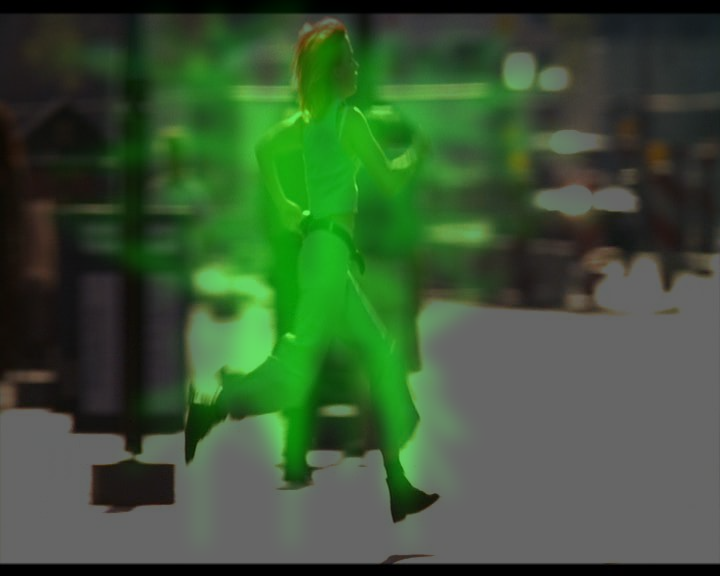
\includegraphics[width=31.6mm]{human_pose/7.png} & 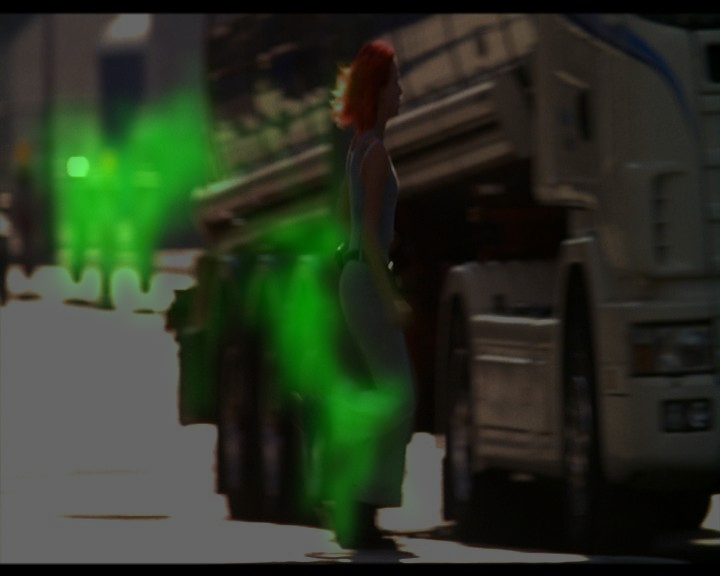
\includegraphics[width=31.6mm]{human_pose/8.png} \\
			(a) & (b)
		\end{tabular}
		\caption{Visualization of best constructed hypotheses. Area, where most hypotheses were found, are highlighted in green. In frame (a) detector find a lot of good hypotheses. In frame (b) detector cannot find a good set of hypotheses.}
		\label{fig:good_bad_hypotheses}
	\end{center}
\end{figure}

The fourth step type allows the inference algorithm to use high-scored poses found in a still frame. It speedups optimization in earlier stages. In figure \ref{fig:good_bad_hypotheses} we demonstrate an area, where the best pose hypotheses were found. In other hand, it makes the inference sensitive to mistakes of human pose detector in a still frame (fig. \ref{fig:good_bad_hypotheses} b). Therefore, we add the first three types of steps to deal with this problem.

\subsubsection{Hidden State Estimation}

As described above, the transition model modifies only joint locations and the scale parameters.
Therefore the joint velocity values should be estimated. We choose the optimal values of the velocity parameters after each type of steps. In other words we chose values of the velocity parameters that maximize the score function:
\[
	V_l = \underset{V}{\mathop{argmax\:}} {Score(Pa)}
\]

Velocities of the different joints are independent given the joint locations in the proposed model of the human pose in a video. Consequently, the velocity parameters of each joints can be estimated separately.

The form of the term $\psi_j(J_t^j, J_{t-1}^j, S_{t-1})$ implies that the function $Score(Pa)$ is factorized accordingly to the graphical model presented in the figure \ref{gm:velocity} given the human joint locations and the scale parameters. Therefore the velocity of each joint can be estimated efficiently.

\begin{figure*}[!t] 
	\begin{center}
		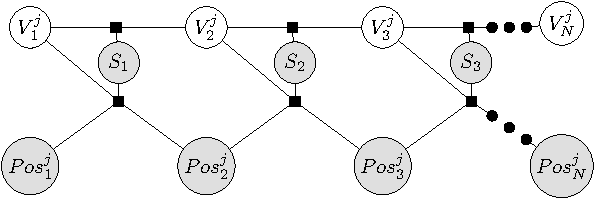
\includegraphics{human_pose/5.pdf}
%		%\beginpgfgraphicnamed{model-simpleModel}
\begin{tikzpicture}

\tikzstyle{myDot} = [circle, fill=black,minimum size=5pt, inner
sep=0pt]

  % Define nodes
  \node[obs]                                  (P1) {$POS_1^j$};
  \node[obs, right=2cm of P1]                 (P2) {$POS_2^j$};
  \node[obs, right=2cm of P2]                 (P3) {$POS_3^j$};
  \node[obs, right=2cm of P3]                 (PN) {$POS_N^j$};
  \node[obs, above=0.9cm of P1, xshift=1.5cm] (S1) {$S_1$};
  \node[obs, above=0.9cm of P2, xshift=1.5cm] (S2) {$S_2$};
  \node[obs, above=0.9cm of P3, xshift=1.5cm] (S3) {$S_3$};
  \node[latent, above=1.5cm of P1]            (V1) {$V_1^j$};
  \node[latent, above=1.5cm of P2]            (V2) {$V_2^j$};
  \node[latent, above=1.5cm of P3]            (V3) {$V_3^j$};
  \node[latent, above=1.5cm of PN]            (VN) {$V_N^j$};
  \node[myDot, right=1.4cm of V3]             (Dot1) {};
  \node[myDot, right=0.10cm of Dot1]          (Dot2) {};
  \node[myDot, right=0.10cm of Dot2]          (Dot3) {};
  \node[myDot, right=1.4cm of V3, yshift=-1.5cm]    (Dot21) {};
  \node[myDot, right=0.10cm of Dot21, yshift=-0.2cm]  (Dot22) {};
  \node[myDot, right=0.10cm of Dot22, yshift=-0.2cm]  (Dot23) {};

  % unary factors
  \factor [below=0.8cm of V1, xshift=1.5cm] {V1-factor}  {} {} {}
  \factor [below=0.8cm of V2, xshift=1.5cm] {V2-factor}  {} {} {}
  \factor [below=0.8cm of V3, xshift=1.5cm] {V3-factor}  {} {} {}
  % pairwise factors
  \factor [right=1cm of V1] {V12-factor}  {} {} {}
  \factor [right=1cm of V2] {V23-factor}  {} {} {}
  \factor [right=1cm of V3] {V3N-factor}  {} {} {}

  %% Connect the nodes
  % unary
  \factoredge {P1, P2, V1, S1} {V1-factor} {}
  \factoredge {P2, P3, V2, S2} {V2-factor} {}
  \factoredge {P3, Dot21, V3, S3} {V3-factor} {}
  \draw (Dot23) -- (PN);
  % paiwise
  \factoredge {V1, V2, S1} {V12-factor} {}
  \factoredge {V2, V3, S2} {V23-factor} {}
  \factoredge {V3, Dot1, S3} {V3N-factor} {}
  \draw (Dot3) -- (VN);

  % Plates
%  \plate {yx} {(x)(y)} {$N$} ;
%  \plate {} {(w)(y)(yx.north west)(yx.south west)} {$M$} ;

\end{tikzpicture}
%\endpgfgraphicnamed
	\end{center}
	\caption{A graphical model for a joint velocity estimation. Nodes of the observed variables are shown in gray.} \label{gm:velocity}
\end{figure*}

We break the term $\phi_j(J_t^j, J_{t-1}^j, S_{t-1})$ into unary and pairwise terms based on the joint velocity parameters (we skips parameters of the terms to simplify description):
\[
\psi_j = \psi_j^u(V_{t-1}^j) + \psi_j^p(V_{t-1}^j, V_t^j)
\]
The unary and the pairwise terms have the following form:
\begin{equation*}
	\begin{aligned}
		\psi_j^u(V_{t-1}^j) &=
			-\frac{{{E^u}_{t}^j}^T {\Sigma_p^p}^{-1} {E^u}_{t}^j} {2 S_{t-1}^2} \\ 
		{E^u}_{t}^j &= \Delta Pos_{t-1}^j - A^u V_{t-1}^j \\
		\Delta Pos_{t}^j &= Pos_{t}^j - A_p^u Pos_{t-1}^j \\
		\psi_j^p &=
			-\frac{{{E^p}_{t}^j}^T {\Sigma_p^v}^{-1} {E^p}_{t}^j} {2 S_{t-1}^2} \\ 
		{E^p}_{t}^j &= V_t^j - A^p V_{t-1}^j \\
		A &= \left[
			\begin{array}{c|c}
				A_p^u  & A^u \\ \hline
				\Theta & A^p
			\end{array}
			\right]
			A_p^u, A^u, A^p \in \mathbb{R}^{2 \times 2}
	\end{aligned}
\end{equation*}

In this form the problem of a posterior velocity estimation is equal to the inference problem in the following Linear Dynamical System:
\begin{equation*}
	\begin{aligned}
		\overline{V}^j &= \underset{V^j}{\mathop{argmax\:}} {p\left(\overline{V}^j | \Delta \overline{Pos}^j
	\right)} \\ 
		\Delta \overline{Pos}_t^j &\sim N(A^u \overline{V}_t^j, \Sigma_p^p) \\
		\overline{V}_t^j &\sim N(A^p \overline{V}_{t-1}^j, \Sigma_p^v) \\
		\overline{V}_1^j &\sim N(\mu_0, \Sigma_0) \\
		\overline{V}_N^j &= A^p \overline{V}_{N-1}^j \\
		\mu_0 &= \Theta_{2\times1} \\
		\Sigma_0 &= \sigma_0 I_{2\times2} \\
		\sigma_0 &\rightarrow \infty
	\end{aligned}
\end{equation*}
where $\Delta \overline{Pos}^j$ is a set of observed normalized velocity values of the human joint, $\overline{V}^j$ is a set of normalized values of the hidden velocity parameters:
\begin{equation*}
	\begin{aligned}
		\Delta \overline{Pos}_t^j &= \frac {\Delta Pos_t^j} {S_t} \\
		\overline{V}_t^j &= \frac {V_t^j} {S_t} \\
	\end{aligned}
\end{equation*}

We use the Kalman filter with the RTS smoother \cite{rauch1965maximum} to estimate the optimal values of the joint velocity.

We simulate a prior distribution on each component of the velocity parameters in the first frame with the normal distribution with dispersion going to infinity. Consequently, it indicates an absence of a prior preferences on the velocity. It implies the following modifications in the Kalman filter:
\begin{equation*}
	\begin{aligned}
		K_1 &= A^{uT} \left(A^u A^{uT}\right)^{-1} \\
		\hat{\mu}_1^j &= K_1 \Delta \overline{Pos}_1^j \\
		\hat{\Sigma}_1^j &= 
		\left(A^{uT} A^u\right)^{-1} A^{uT} \Sigma_p^p \left(A^u A^{uT}\right)^{-1} A^u
	\end{aligned}
\end{equation*}

We estimate the values of $\overline{V}_t^j$ by the Viterbi algorithm \cite{viterbi1967error} for LDS (alg. \ref{alg:velocity}). It means that the original velocity parameters has the following estimations:
\[
V_t^j|\Delta\overline{Pos}^j \sim N\left(S_t\mu_t^j, S_t^2 \Sigma_t^j \right)
\]

\begin{algorithm}[!t]
	\KwData{$\Delta \overline{Pos}_1^j, \dots, \Delta \overline{Pos}_{N-1}^j$ are the observed data, $(A^u, A^p, \Sigma_p^p, \Sigma_p^v)$ are the model parameters}
	\KwResult{$\mu_1^j, \dots, \mu_{N}^j, \Sigma_1^j, \dots, \Sigma_N^j$}
	
	// the Kalman filter\;
	$K_1 = A^{uT} \left(A^u A^{uT}\right)^{-1}$\;
	$\hat{\mu}_1^j = K_1 \Delta \overline{Pos}_1^j $\;
	$\hat{\Sigma}_1^j =
	\left(A^{uT} A^u\right)^{-1} A^{uT} \Sigma_p^p \left(A^u A^{uT}\right)^{-1} A^u$ \;
	\For{t = 2,\dots, N-1}{
		$\tilde{\Sigma}_{t-1} = A^p \hat{\Sigma}_{t-1}^j A^{pT} + \Sigma_p^v$\;
		$K_{t} = \tilde{\Sigma}_{t-1} A^{uT} (A^u \tilde{\Sigma}_{t-1} A^{uT} + \Sigma_p^p)^{-1}$\;
		$\hat{\mu}_t^j = A^p \hat{\mu}_{t-1}^j + K_t \left( \Delta \overline{Pos}_t^j -
		A^u A^p \hat{\mu}_{t-1}^j \right)$\;
		$\hat{\Sigma}_t^j = (I - K_{t} A^u) \tilde{\Sigma}_{t-1}$ \;
	}
	
	// The RTS smoother\;
	$\mu_{N-1}^j = \hat{\mu}_{N-1}^j$\;
	$\Sigma_{N-1}^j = \hat{\Sigma_{N-1}^j}$\;
	\For {t = N-2,\dots,1}{
		$K_t=\hat{\Sigma}_t^j A^p \tilde{\Sigma}_t^{-1}$\;
		$\mu_t^j = \hat{\mu}_t^j + K_t(\mu_{t+1}^j - A^p \hat{\mu}_t^j)$\;
		$\Sigma_t^j = \hat{\Sigma}_t^j + K_t (\Sigma_{t+1}^j - \tilde{\Sigma}_t^j)K_t^T$\;
	}
	$\mu_N = A^p \mu_{N-1}^j$\;
	$\Sigma_N^j = \Sigma_p^v + A^p \Sigma_{N-1}^j A^{pT}$\;
	\caption{An algorithm of a joint velocity $V^j$ estimation.} \label{alg:velocity}
\end{algorithm}

\begin{algorithm}[H]
	\SetAlgoLined %% Это соединяет линиями логические части 
	%% алгоритма типа if-then-else
	
	\KwData{ $I, \tilde{P}, N$} %% здесь можно указать исходные параметры
	
	\KwResult{ $P$ } %% результат работы программы
	
	$\tilde{V} \leftarrow \argmax{E(V|\tilde{P})}$;
	
	$H_0 \leftarrow \left(\tilde{P}, \tilde{V} \right)$;
	
	\For{$i=\overline{1,N}$}{
		
		$i \leftarrow sample\_step()$;
		
		$\widehat{P} \leftarrow apply\_step(H_{i-1}, k)$;
		
		$\widehat{V} \leftarrow \argmin{E(V|\widehat{P})}$;
		
		$H_i \leftarrow choose\_next(H_{i-1}, (\widehat{P}, \widehat{V}))$;
		
	}

	$P \leftarrow \argmin_i{E(H_i)}$;
	
	\caption{Алгоритм сэмплирования для построения позы человека в видео.}
	\label{alg:generalHM}
\end{algorithm}

\subsection{Доказательство сходимости}
\subsection{Доказательство корректности}
\subsection{Оценка сложности}
\section{Экспериментальная оценка}
\subsection{Описание тестовых данных}
\subsection{Анализ результатов}
